
Chương này, trình bày một số nội dung về dữ liệu và những công cụ được
sử dụng trong quá trình thực nghiệm, đánh giá kết quả thực nghiệm đã 
làm được cũng như khả năng ứng dụng và hướng phát triển của đề tài 
trong tương lai. Qua đó đưa ra những nhận xét, đánh giá và kết luận 
chung cho đề tài.

\section{Dữ liệu thực nghiệm}

Để tiến hành thực nghiệm những nội dung nghiên cứu lý thuyết trong đề
tài, tôi đã sử dụng hai nguồn dữ liệu chính để làm thực nghiệm. Một
nguồn là dữ liệu của trò chơi Code Hunt, nguồn dữ liệu còn lại do tôi
tự xây dựng.

Code Hunt là một game về lập trình, được sử dụng cho
các cuộc thi viết mã và thực hành các kỹ năng lập trình do Microsoft
phát triển. Code Hunt dựa trên công cụ Pex, ứng dụng kỹ thuật DSE khám
phá các nhánh đường đi của chương trình để suy ra giá trị đầu vào có
độ phủ cao. Dữ liệu trong trò chơi Code Hunt là một tập hợp những
chương trình con, tương ứng mỗi chương trình con là những câu hỏi được
trình bày như một bài kiểm tra. Người chơi phải chọn câu hỏi và trả
lời câu hỏi bằng cách viết một đoạn mã sao cho kết quả trùng với
đáp án của câu hỏi. Hiện nay Code Hunt đã được hơn 350.000 người chơi
sử dụng tính đến tháng 8 năm 2016 \cite{CodeHunt}. Dữ liệu từ các cuộc 
thi gần đây đã được công khai, cho phép những người quan tâm đến 
Code Hunt tải về để phân tích và nghiên cứu trong cộng đồng giáo dục.

\label{sec:data}
\begin{center}
  \begin{figure}[H]
    \begin{center}
      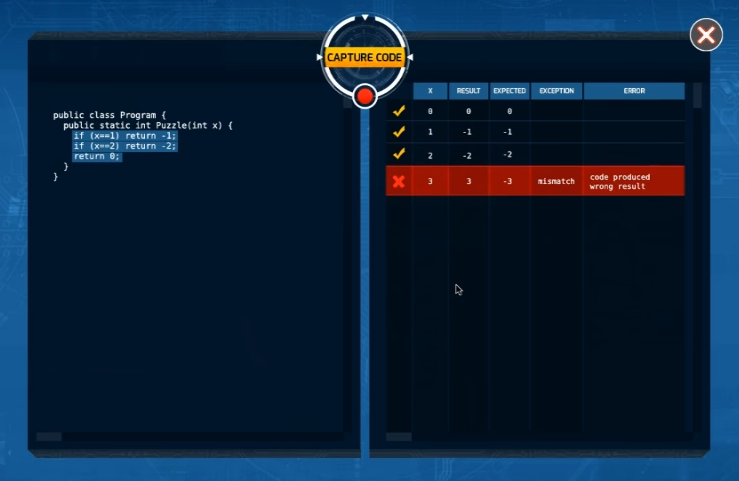
\includegraphics[scale=.5]{codehunt.png}
    \end{center}
    \caption{Giao diện viết chương trình của Code Hunt}
    \label{codehunt2}
  \end{figure}
\end{center}

Tập dữ liệu Code Hunt là một tập dữ liệu chứa các chương trình do sinh 
viên trên toàn thế giới viết khi tham gia trò chơi, với 250 người sử dụng, 
24 câu hỏi và khoảng 13.000 chương trình được sinh viên thực hiện trên 2 
ngôn ngữ là Java và C\#. Để có thể sử dụng tập dữ liệu Code Hunt trong 
thực nghiệm, tôi đã thực hiện kiểm tra và loại bỏ một số chương trình bị 
lỗi và không phù hợp với đề tài.

\section{Công cụ dùng trong thực nghiệm}
%Phần này trình bày những công cụ được sử dụng để triển khai thực nghiệm như: công cụ sinh dữ liệu kiểm thử, môi trường lập trình, \dots

Trong quá trình làm thực nghiệm, tôi đã sử dụng một số công cụ để tạo ứng 
dụng minh họa cho các phép đo độ tương tự hành vi của chương chình.

\subsection{Microsoft Visual studio}
Microsoft Visual Studio là một sản phẩm của hãng Microsoft. Nó được sử dụng 
để phát triển chương trình máy tính cho Microsoft Windows, cũng như các 
trang web, các ứng dụng web và các dịch vụ web. Microsoft Visual Studio 
sử dụng nền tảng phát triển phần mềm của Microsoft như Windows API, Windows 
Forms, Windows Presentation Foundation, Windows Store và Microsoft Silverlight. 

Visual Studio hỗ trợ nhiều ngôn ngữ lập trình khác nhau và cho phép trình biên 
tập mã và gỡ lỗi để hỗ trợ (mức độ khác nhau) hầu như mọi ngôn ngữ lập trình. 
Các ngôn ngữ tích hợp gồm có C, C++ và C++/CLI (thông qua Visual C++), VB.NET 
(thông qua Visual Basic.NET), C\#  (thông qua Visual C\#) và F\# 
(như của Visual Studio 2010). Hỗ trợ cho các ngôn ngữ khác như J++/J\#, Python 
và Ruby thông qua dịch vụ cài đặt riêng rẽ. Nó cũng hỗ trợ XML/XSLT, 
HTML/XHTML, JavaScript và CSS.

Trong luận văn này, tôi sử dụng chủ yếu là ngôn ngữ lập trình C\# để viết ứng 
dụng minh họa. Ngôn ngữ lập trình này là một ngôn ngữ lập trình hiện đại, được 
phát triển bởi Anders Hejlsberg cùng nhóm phát triển .Net Framework của Microsoft 
và được phê duyệt bởi European Computer Manufacturers Association (ECMA) và 
International Standards Organization (ISO). Mã nguồn C\# là các tập tin *.cs 
được trình biên dịch Compiler biên dịch thành các file *.dll hoặc *.exe, sau 
đó các file này được các hệ thống thông dịch CLR trên điều hành thông dịch qua 
mã máy và dùng kỹ thuật JIT (just-in-time) để tăng tốc độ. Hình \ref{fig:ProcessCompile} 
mô tả quá trình biên dịch một file *.cs.


\begin{figure}[H]	
	\begin{center}
	  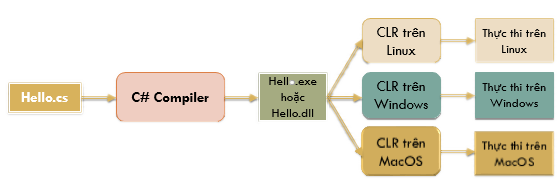
\includegraphics[scale=.7]{quatrinhthongdich.png}
	\end{center}
	\caption{Quá trình biên dịch chương trình trong C\#}
	\label{fig:ProcessCompile}
\end{figure}


C\# có thể tạo ra được nhiều loại ứng dụng, trong đó có 3 kiểu phổ biến được 
nhiều người sử dụng nhất đó là: Console, Window và ứng dụng Web. 

\subsection{Công cụ sinh dữ liệu thử Pex}
Công cụ Pex là một sản phẩm của Microsoft được xây dựng và phát 
triển dựa trên kỹ thuật DSE. Trong Visual Stuio, Pex đã được tích hợp 
như một Add-in \cite{tillmann2014transferring}, có thể tạo ra các test case kết hợp với các bộ kiểm 
thử khác nhau như NUnit và MSTest. Về bản chất công cụ Pex là một công cụ hỗ trợ 
kỹ thuật kiểm thử hộp trắng (white-box) ghi nhận lại các ràng buộc tại các nút 
rẽ nhánh của chương trình, phủ định lại các ràng buộc này và sinh ra các đầu 
vào có thể phủ hết các nhánh của chương trình. Hình \ref{fig:ModelPex}\cite{tillmann2013teaching} mô tả 
mô hình hoạt động và ứng dụng của công cụ Pex.

\begin{figure}[H]	
	\begin{center}
		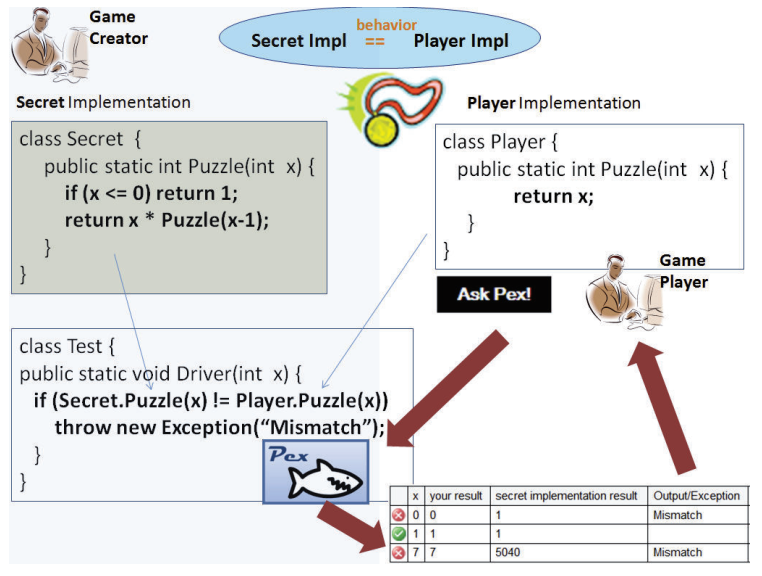
\includegraphics[scale=.6]{pex.png}
	\end{center}
	\caption{Mô hình hoạt động của công cụ Pex}
	\label{fig:ModelPex}	
\end{figure}

Cũng như với Unit Test, chúng ta có thể sử dụng công cụ Pex để viết 
các lớp kiểm thử với nhiều ca kiểm thử khác nhau, nhưng Pex chỉ 
thực thi được một ca kiểm thử trong mỗi lần chạy.

\section{Đánh giá kết quả thực nghiệm}

Trong nội dung Chương \ref{chap:behaviors} và Chương \ref{chap:method} của đề tài, 
đã trình bày một số lý thuyết về kiểm thử phần mềm, kỹ thuật sinh dữ liệu thử nghiệm, 
và các phép đo độ tương tự hành vi của chương trình RS, SSE, PSE. Áp dụng những
lý thuyết trên, tôi thực nghiệm bằng cách xây dựng một ứng dụng để mô tả
quá trình hoạt động của các phép đo, và đánh giá kết quả các phép đo. 
Kết quả thực nghiệm đạt được như Hình \ref{fig:frmMain}

\begin{figure}[H]	
	\begin{center}
	 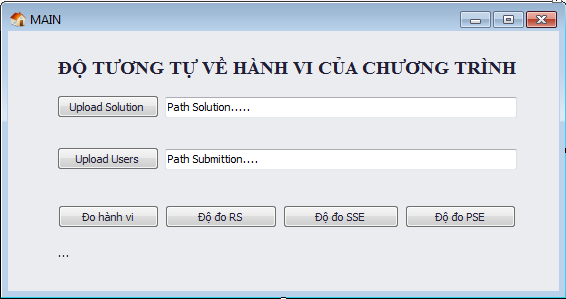
\includegraphics[scale=.8]{main.png}
	\end{center}
	\caption{Giao diện màn hình chính của ứng dụng}
	\label{fig:frmMain}
\end{figure}

Hai nút đầu tiên, cho phép chúng ta chọn chương trình tham chiếu và chọn files cần 
tính độ tương tự. Bên dưới là nút đo hành vi của chương trình, và các nút tính 
toán độ tương tự hành vi của chương trình theo các phép đo RS, SSE và PSE.

Để mô tả hoạt động của ứng dụng, tôi thực hiện chọn một mã lệnh mẫu làm chương 
trình tham chiếu với Mã lệnh \ref{lst:pro-reference} và hai chương trình cần 
tính độ tương tự với Mã lệnh \ref{lst:pro-user1} và Mã lệnh \ref{lst:pro-user2}.

\lstinputlisting[label={lst:pro-reference}, caption = {Chương trình tham chiếu}]{solution.cs}
\lstinputlisting[label={lst:pro-user1}, caption = {Chương trình của sinh viên thứ nhất}]{user1.cs}
\lstinputlisting[label={lst:pro-user2}, caption = {Chương trình của sinh viên thứ hai}]{user2.cs}


\subsection{Độ tương tự hành vi của chương trình theo phép đo RS}
Dựa vào kết quả độ đo RS ở Hình \ref{fig:result-RS}, chúng ta có một tập các 
giá trị đầu vào với $ 200 $ phần tử được sinh ngẫu nghiên từ miền giá trị đầu vào 
kiểu \texttt{int} của chương trình. Kết quả độ tương tự hành vi chương trình của 
sinh viên với chương trình tham chiếu theo phép đo RS lần lượt đều bằng $ 1 $, 
Với kết quả này, hai chương trình của sinh viên được xem là tương đương với 
chương trình tham chiếu. 

\begin{figure}[H]	
	\begin{center}
		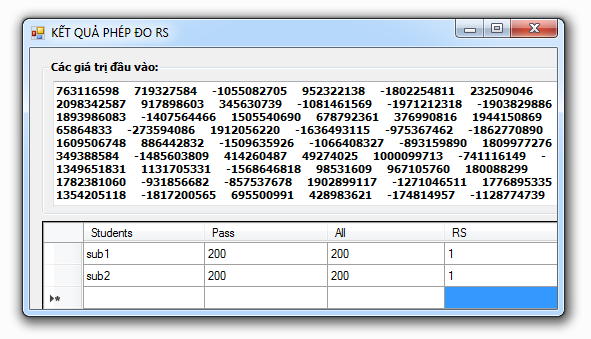
\includegraphics[scale=.8]{kq_rs.png}
	\end{center}
	\caption{Độ tương tự hành vi của chương trình sử dụng phép đo RS}
	\label{fig:result-RS}
\end{figure}


Trong khi đó, phân tích mã lệnh chương trình của hai sinh viên với mã lệnh chương 
trình tham chiếu ta thấy tất cả đều có cùng tham số vào kiểu \texttt{int} cùng 
tính toán và trả về kết quả $ y $ phụ thuộc vào $ x $. Mã lệnh \ref{lst:pro-user1} 
của sinh viên thứ nhất khác với mã lệnh chương trình tham chiếu với hành vi 
\textit{if (x == 2) return y *= 4} và Mã lệnh \ref{lst:pro-user2} của sinh viên 
thứ hai khác với mã lệnh chương trình tham chiếu với hành vi 
\textit{if (x == 2) return y *= 4} và \textit{if (x == 3) return y *= 6}.

Vì vậy, kết quả độ tương tự hành vi chương trình của hai sinh viên với chương trình 
tham chiếu theo phép đo RS cho kết quả tương đối, giá trị đầu vào thử nghiệm được 
lấy ngẫu nhiên từ miền vào của các chương trình không phủ hết đường đi trong chương 
trình của hai sinh viên và chương trình tham chiếu.

\subsection{Độ tương tự hành vi của chương trình theo phép đo SSE}

Phân tích chương trình tham chiếu với kỹ thuật DSE chúng ta có tập các đầu vào thử 
nghiệm là $(0, 1, 2)$. Khi thực thi chương trình của hai sinh viên và chương trình 
tham chiếu với tập các đầu vào này, kết quả đầu ra chương trình của hai sinh viên 
có $ 2 $ kết quả trên tổng số 3 kết quả giống với chương trình tham chiếu, kết quả 
là $0,66$ như Hình \ref{fig:results-SSE}. Chúng ta thấy kết quả này đã thay đổi so 
với kết quả của phép đo RS (kết quả phép đo RS bằng $ 1 $). Tập các đầu vào thử 
nghiệm được tạo ra bởi kỹ thuật DSE có độ phủ cao, có thể phủ hết các nhánh của 
chương trình tham chiếu. Do vậy phép đo SSE cho kết quả chính xác hơn phép đo RS.

\begin{figure}[H]
	\begin{center}
		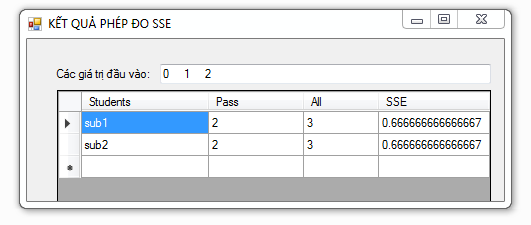
\includegraphics[scale=.8]{kq_sse.png}
	\end{center}
	\caption{Độ tương tự hành vi của chương trình theo phép đo SSE}
	\label{fig:results-SSE}
\end{figure}

Tuy nhiên, phép đo SSE lại không quan tâm đến hành vi của chương trình cần tính để 
tạo ra các đầu vào thử nghiệm có khả năng phủ hết các nhánh đường đi trong chương 
trình của sinh viên. Các dữ liệu đầu vào trong trường hợp này không phủ hết được 
nhánh \texttt{(if(x==3) return y*=6)} trong chương trình của sinh viên thứ hai.

\subsection{Độ tương tự hành vi của chương trình theo phép đo PSE}
Dựa trên kết quả Hình \ref{fig:result-PSE}, chúng ta thấy kết quả độ tương tự hành 
vi chương trình của sinh viên thứ nhất với chương trình tham chiếu theo phép đo PSE 
giống với kết quả của phép đo SSE \textit{(cả hai phép đo đều bằng $ 0.66 $)} và tập 
dữ liệu vào được tạo bởi DSE trên chương trình hợp thành của hai chương trình 
$ (0, 1, 2) $ cũng không thay đổi so với phép đo SSE.

\begin{figure}[H]	
	\begin{center}
		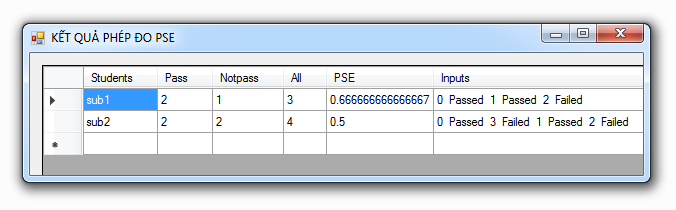
\includegraphics[scale=.7]{kq_pse.png}
	\end{center}
	\caption{Độ tương tự hành vi của chương trình theo phép đo PSE}	
	\label{fig:result-PSE}	
\end{figure}

Nhưng độ tương tự hành vi chương trình của sinh viên thứ hai với chương trình tham 
chiếu theo phép đo PSE đã thay đổi bằng $ 0.5 $, kết quả này nhỏ hơn so với kết quả 
$ 0.66 $ của phép đo SSE. Phép đo PSE cũng đã tạo ra tập dữ liệu vào dựa trên chương 
trình hợp thành với $ 4 $ phần tử là $ (0, 3, 1, 2) $ nhiều hơn tập đầu vào do phép 
đo SSE tạo ra $ 1 $ phần tử.

Dựa trên chương trình hợp thành, DSE đã tạo ra tập đầu vào có độ phủ cao, có thể thực 
thi hết các nhánh của chương trình tham chiếu và chương trình của sinh viên thứ hai. 
Kết quả độ tương tự hành vi của chương trình của hai sinh viên với chương trình tham 
chiếu theo phép đo PSE cho kết quả tương đối chính xác.

\section{Khả năng ứng dụng}

Các kỹ thuật đo độ tương tự trình bày trong đề tài này có thể áp dụng
được trong nhiều lĩnh vực, nhưng chủ yếu tập trung vào giáo dục, chương trình đào 
tạo lập trình viên, hay đào tạo kỹ sư phần mềm... Một
số ứng dụng thực tế có thể phát triển trong tương lai như:

\textbf{\textit{Đánh giá tiến bộ trong lập trình:}} Theo dõi sự tiến
bộ trong học tập là một việc quan trọng, mà ngay cả với giảng viên và
sinh viên. Có nhiều tiêu chí đánh giá sự tiến bộ trong học tập của
sinh viên, trong đó tiêu chí về điểm số là một trong những tiêu chí cơ
bản nhất. Một bảng điểm thống kê điểm số, thành tích học tập của sinh
viên sẽ thể hiện được sự tiến bộ của sinh viên trong học tập. Một ứng
dụng hỗ trợ chấm điểm, lưu trữ, thống kê và đánh giá điểm số của sinh
viên là sẽ là một công cụ hỗ trợ đắc lực cho giảng viên trong công tác
quản lý của mình. Nếu số liệu thống kê kết quả các bài kiểm tra của
sinh viên ngày càng cao, chứng tỏ sinh viên nắm được nội dung và kiến
thức của chương trình đào tạo, và kết quả tốt sẽ là một động lực giúp
cho sinh viên thêm tự tin, đam mê công việc học tập của mình. Ngược
lại, nếu một sinh viên có điểm số ngày càng thấp đi, chứng tỏ sinh
viên đang có vấn đề trong kiến thức của của mình, lúc này tốt nhất
sinh viên nên dừng lại và kiểm tra xem vấn đề mình đang gặp phải.

\textit{\textbf{Xếp hạng tự động:}} Công việc chấm điểm, phân loại và
xếp hạng các bài kiểm tra của sinh viên cũng là một công việc tốn
không ít công sức của giảng viên. Để giảm bớt gánh nặng cho giảng
viên, chúng ta có thể sử dụng kết quả các phép đo trên từng bài tập
của sinh viên như một phương pháp hỗ trợ công việc chấm điểm của từng
sinh viên. Sự giống nhau về hành vi giữa chương trình của sinh viên và
chương trình tham chiếu có thể là một yếu tố để phân loại sinh
viên. Độ tương tự càng cao thì điểm số càng cao, các chỉ số này dựa
hoàn toàn trên ngữ nghĩa của chương trình. Cách tiếp cận này giải
quyết được các giới hạn trong trường hợp chương trình của sinh viên
giống với chương trình tham chiếu, nhưng khác nhau về ngữ nghĩa. Các
kết quả trong việc xếp hạng tự động sẽ giúp tiết kiệm được thời gian
và giảng viên có thể đưa ra giải pháp giúp những sinh viên có điểm số
thấp khắc phục được hạn chế đang gặp phải.

\textit{\textbf{Gợi ý giải pháp lập trình:}} Thông thường, sinh viên
viết code mới thực hiện chạy chương trình, lúc này sinh viên
mới biết được kết quả đoạn code vừa thực hiện. Để hỗ trợ sinh viên
viết code được tốt hơn, nếu như có một công cụ hỗ trợ kiểm tra theo
thời gian thực và gửi thông báo lỗi nếu sinh viên viết code sai cú
pháp hoặc chương trình bị lỗi không thể thực thi được. Ngoài ra, công
cụ sẽ gợi ý giải pháp lập trình cho sinh viên bằng hình thức tự động
tính toán thông báo kết quả các tham số đầu vào và đầu ra của chương
trình so với chương trình được tham chiếu, đưa ra các số liệu về độ
tương tự hành vi của chương trình.

\section{Kết luận}
Qua quá trình nghiên cứu đề tài, có thể thấy rằng việc sử dụng một 
công cụ hỗ trợ để đo độ tương tự hành vi chương trình phục vụ trong 
việc dạy và học tại các trường đào tạo lập trình viên là rất cần 
thiết. Công cụ hỗ trợ không chỉ giúp giảng viên tiết kiệm được thời 
gian trong việc đọc và đánh giá các đoạn mã lệnh do sinh viên viết. 
Bên cạnh đó, công cụ còn hỗ trợ cho giảng viên trong việc đánh giá 
xếp loại học lực của sinh viên thông qua kết quả độ tương tự hành vi 
của chương trình sinh viên với chương trình tham chiếu. Sinh viên cũng  
có thể sử dụng công cụ này trong việc thực hành kỹ năng lập trình 
và giải các bài tập do giảng viên đưa ra. 

Một công cụ hỗ trợ để đo độ tương tự hành vi chương trình cần tính
với chương trình tham chiếu phải đảm bảo thực thi nhanh và có kết quả 
chính xác. Tuy nhiên, các phép đo độ tương tự hành vi của chương trình 
được nghiên cứu trong đề tài đều có ưu điểm và hạn chế riêng. Phép đo RS có 
ưu điểm là đánh giá khách quan, chương trình có tốc độ xử lý nhanh, ít tốn 
tài nguyên máy tính, nhưng phép đo RS có hạn chế khi kết quả phép đo 
chỉ ở mức độ tương đối vì phép đo không quan tâm đến hành vi 
của chương trình, chỉ quan tâm đến dữ liệu vào và ra của chương trình.
Phép đo SSE sử dụng kỹ thuật DSE để sinh ra tập các giá trị đầu vào của 
chương trình, các giá trị trong tập đầu vào này có khả năng phủ tất cả 
nhánh của chương trình tham chiếu, vì vậy phép đo SSE cho kết quả độ tương 
tự hành vi của chương trình chính xác hơn phép đo RS. Tuy nhiên, phép đo 
SSE vẫn có hạn chế khi không quan tâm đến hành vi của chương trình cần 
tính, tập đầu vào của phép đo SSE không phủ được tất cả các nhánh của 
chương trình cần phân tích. Để giải quyết hạn chế của phép đo SSE, phép đo 
PSE sử dụng kỹ thuật DSE để tạo tập giá trị đầu vào trên chương trình hợp 
thành của chương tình cần tính và chương trình tham chiếu. Tập các giá trị 
đầu vào này có khả năng phủ tất cả các nhánh đường đi trên cả hai chương 
trình. Kết quả của phép đo PSE tương đối chính xác và tốt hơn kết quả của 
phép đo SSE, nhưng phép đo PSE lại tốn nhiều tài nguyên máy tính và thời 
gian thực thi lâu hơn phép đo SSE.

Từ các kết quả đã đạt được, tương lai đề tài có thể phát triển thành 
một ứng dụng hoàn thiện, bằng cách cải tiến các kỹ thuật đo để kết quả 
các phép đo được chính xác hơn và nhạy hơn. Bổ sung thêm một số chức năng 
như phân loại, xếp hạng tự động đánh giá kết quả học tập của sinh viên... 
Ngoài ra, để ứng dụng được nhiều người quan tâm hơn thì ứng dụng phải 
đơn giản, thân thiện và phải hỗ trợ một số ngôn ngữ lập trình phổ biến như Java, C++... 

Quá trình nghiên cứu những kiến thức cơ sở của đề tài và tiến hành làm 
thực nghiệm, bản thân tôi cũng gặp rất nhiều khó khăn như: Lượng kiến thức 
cơ sở cần phải nghiên cứu tương đối nhiều; bản thân thiếu kinh nghiệm trong 
việc thực hiện các đề tài... Tuy nhiên, nhờ sự động viên và giúp đỡ của bạn 
bè, gia đình, cùng với sự giúp đỡ của giáo viên hướng dẫn tôi đã hoàn 
thành luận văn, đáp ứng được các yêu cầu đã đề ra.


%%% Local Variables:
%%% mode: latex
%%% TeX-master: "Main"
%%% End:
